
\section{Spatial Closure based on the HO Solution}
\label{sec:spat_clos}

This sections describes an alternative spatial closure to the LO equations based on 
a parametric relation from the HO solution. In addition to estimating the angular
consistency terms, the HO intensity estimates a relation between volume and face-averaged
intensities to eliminate the remaining unknowns from the equations.  In the remainder of
this section, we will motivate the HO spatial closure by manipulating a half-range balance
equations to form a single unknown for each cell and half range.  We will then discuss
the forms of HO spatial closures investigated, based on modifications to standard spatial closures.

\subsection{Motivation}

A half-range balance equation for $\mu>0$ is formed by adding the
exact $L$ and
$R$ radiation moment equations given by
Eq.~\eqref{eq:exact_lmomp}~and~\eqref{eq:exact_rmomp}, i.e.,
\begin{equation}\label{eq:hr_bal}
    \mu^+_{i+1/2}\phi_{i+1/2}^+ - \mu^+_{i-1/2}\phi_{i-1/2}^+ +
    {\sigma_{a,i}h_i} \phi_i^+ = \frac{h_i}{2} q_i,
\end{equation}
where $q_i$ represents the cell-averaged emission source.  In the HOLO algorithm, after
estimating the consistency terms $\mu_{i\pm1/2}^+$ upwinding the inflow term
$\phi_{i-1/2}^+$, an additional equation is needed to eliminate the outflow $\phi_{i+1/2}^+$ to produce an
equation for a single unknown $\phi_{i}^+$.  Standard spatial discretizations techniques
use a fixed approximation for all cells to eliminate the outflow in terms of other
unknowns.  Alternatively, the HO solution can be used to estimate a parametric relation
between the other unknowns and the outflow, i.e.,
\begin{equation}\label{eq:ho_clos}
    \phi_{i+1/2}^+ = f(\gamma^{+,HO}_i, \phi_i^+, \phi_{x,i}^+, \phi_{i-1/2}^+),
\end{equation}
where $\gamma^{HO,+}_i$ is a local constant to be estimated with the HO solution and $f$ is some
function of some number of the input
variables.  The ECMC solution can provide all of the unknowns in the above equation, so
the value of $\gamma^{HO}_i$ can be determined directly. 

If the problem were linear, or the nonlinear problem was fully converged,
then application of this closure can ensure that the HO and LO equations produce the same
moments, preserving the HO accuracy.  To produce the
same moments, the HO solution must also satisfy the local balance equation, e.g.,
Eq.~\eqref{eq:hr_bal}.  Then the LO equations and HO equations must have the same moments
to satisfy both Eq.~\eqref{eq:ho_clos} and Eq.~\eqref{eq:hr_bal}, upon nonlinear
convergence. If any higher moments are introduced through the spatial closure,
then the HO solution must also satisfy the same relations as the LO equations.  For example, both the LO and HO equation must satisfy the
first moment equation in space if the closure is a function of the first moment.  

As TRT problems are non-linear (i.e., scattering or thermal emission are included in
$q$), the moments will only be preserved upon non-linear convergence of the source.  The
nonlinearity introduces the possibility for stability
issues, particularly with MC noise.  However, we have already consistently formed angular consistency terms, so the
the spatial closure should be more stable than introducing other terms, such as
in NDA methods~\cite{rmc,holo,willert}. 





\subsection{Choice of Spatial Closure}
\label{sec:spat_clos_options}

We will
explore two different closure relations: a scaled slope, i.e.,
\begin{equation}\label{eq:cl_slope}
    \phi_{i\pm1/2}^\pm = \phi_i^+ \pm \gamma_i \phi_{x,i}^+
\end{equation}
and a scaled average
\begin{equation}\label{eq:cl_avg}
    \phi_{i\pm1/2}^\pm = \gamma_i \phi_i^+ \pm \phi_{x,i}^+,
\end{equation}
where a value of $\gamma_i = 1$ produces the standard linear discontinuous expressions for
the extrapolated outflows.  

We now use the HO solution to estimate $\gamma_i$. The MC solution must be modified
to tally the solution on faces. For example, the LO equations for
moments at $k+1$ use closure parameters evaluated at $k+1/2$ as
\begin{equation}
    \gamma_i^{+,k+1/2} = \frac{\phi_{i+1/2}^{+,HO,k+1/2} -
    \phi_{x,i}^{+,HO,k+1/2}}{\phi_i^{+,HO,k+1/2}},
\end{equation}
for the scaled-average closure.  For this closure, as the slope goes to zero this expression
becomes undefined.  In cells where the slope is $O(10^{-13} \psi_i)$, we use $\gamma_i=1$.
For the problems tested, no issues have occurred with this closure, even $\gamma$
can become very large for common, small values of $|\psi^x/\psi_i|$.  This is because in
such regions the solution is changing minimally anyways. 
The main benefit of this closure is it allows for values of $\gamma$ that are
equivalent to step ($\gamma_i=0$) and lumped ($\gamma_i=1/3$) closures.

To solve the LO equations, the expression for the outflow face term is substituted in each equation, using the
$\gamma_i$ estimated from the HO solution. There is a spatial closure parameter for each
half-range, for each cell.
For instance, the positive balance equation becomes
\begin{equation}
    \overline\mu^+_{i+1/2}\left( \gamma_i^{+,HO} \phi_i^+ + \phi_{x,i}^+ \right) - \overline\mu^+_{i-1/2}\phi_{i+1/2}^+ +
    \frac{\sigma_{a,i}h_i}{2} \phi_i^+ = \frac{h_i}{2} q_i,
    \label{eqn:clsd_posbal}
\end{equation}
noting that $\phi_i^+$ and $\phi_{x,i}^+$ remain as unknowns.  Our LO system is formulated in terms of $L$ and $R$ moments, rather than the average and
slope.  Thus, the parametric functions are expressed in terms of the $L$ and $R$
unknowns, using the relations given in App.~\ref{app:lo_mom_relations}.  


\subsection{The Doubly-Discontinuous Trial Space}

The ECMC algorithm is modified to also include a LDD trial space which allows for estimate
of the face solution~\cite{sec:ldd_mc}.

Because of the temperature unknowns and the HO scattering source representation, a
representation on the interior of the cell for the temperature and intensity is needed.
However, the outflow from the cell is now a parametric (i.e., non linear)
extrapolation of the interior moments. Thus, we introduce a linear doubly
discontinuous (LDD) trial space for the half-range intensities, which is depicted in Fig.~\ref{fig:ldd_space}.
The linear relation on the interior of the cell preserves the $L$ and $R$ moments of the
solution.  The temperature is still represented with a linear interpolant of $T^4$ and
$T$.  This trial space has an extra unknown in each cell, for each direction, which is eliminated from the system
with the HO spatial closure.  For the initial LO solve, the outflow is assumed continuous, using the standard
upwinding and LD representation.  With the outflow term eliminated, the equations
have the same numerical complexity as the LD equations.  The linear representation for the
interior solution and the emission source should preserve the equilibrium diffusion limit,
as long as the HO spatial closure is sufficiently estimated.

In the case of strong gradients, the interior representation could be driven
negative.  Thus, we use the lumped expression to to define the linear representation.  For
example, the lumped emission source is
\begin{equation}
    T = \mom{T}_{L,i}^4 b_{L,i}(x) + \mom{T}_{R,i}^4 b_{R,i}(x) , \quad x\in(\xl,\xr)
\end{equation}
This expression is positive as long as the moments are positive, which is true for
physical solutions.  If the lagged, MC spatial closure produces an outflow from a cell that is
negative, then these moments could become negative.  In such cases, we force that cell to
use a standard lumped relation for the moment equations, with no discontinuity at the
outflow.  

During the Newton solve, once new half-range
intensities are determined, the temperatures are updated using the moment same moment
equations given by Eq.~\eqref{}. This can be confusing because the slope moment,
e.g., $\psi_{x,i}^\pm$, does not strictly correspond to the slope in the typical since.
We have modified it.  This is the same as the lumped closure relation using
$\gamma_i=1/3$, where we are preserving the average moment exactly, but only second order
accurate in the slope.


\begin{figure}[H]
    \centering
    {\resizebox{0.5\textwidth}{!}{
        \begin{tikzpicture}[scale=0.62, every node/.style={transform shape}]
            \draw (1.0,4.0) node[fill,circle,inner sep=0pt,minimum
            size=4.2pt] {};
            \draw [->] (1.6,4.25) -- (2.4,4.25) node[anchor=west] {$\mu$};
            \draw (1.0,0.4) -- (1.0,0.6) node[below, pos=0.4] {$x_{i-1/2}$};
            \draw (5.90,0.4) -- (5.90,0.6) node[below, pos=0.4] {$x_{i+1/2}$};
            \node at (3.6,3.06) {$\phi^+(x)$};
            \draw [thick] (1.0,0.5) -- (5.9,0.5) node[anchor=north west] {};
            \filldraw[color=black, fill=white] (1,3.1250) circle (2.1pt);
            \draw (1.0,3.125) -- (5.90,2.120);
            \filldraw[color=cyan, fill=white] (5.9,2.120) circle (2.1pt);
            \draw (5.9,3.0) node[cyan,fill,circle,inner sep=0pt,minimum size=4.2pt] {};
        \end{tikzpicture}
    }}
    \caption{Linear doubly-discontinous representation for mean intensity in LO equations}
    \label{fig:ldd_space}
\end{figure}

Poor statistics for the face tallies may result in this trial space producing less
accurate results compared to the standard LDFE solution, at least for sufficiently fine meshes where LD
can accurately represent the solution.  Although the closure will be applied everywhere,
we expect the greatest improvement in accuracy for cells where the LDFE trial space
produces a negative solution.

\subsection{Issues with ECMC}

  There are
several issues with ECMC that cause this to not be true, even for a linear problem.
With ECMC, global and, particularly, local energy balance are not preserved.  There
are source biasing techniques for standard MC (e.g., systematic
sampling) that exactly preserve the zeroth moment of the
source~\cite{shultis_mc,wollaber_review}). 
However, because we have to reconstruct the bilnear moment
of $x$ and $\mu$, the consistency terms do not exactly preserve the first moment
equation.  One final reason is that the analog treatment of absorption for particles below
the weight cutoff (e.g., see Sec.~\ref{sec:tallies}) results in $\sigma_a \phi^{HO}_i$ and the amount
of energy removed from a cell during MC transport to not be equal, due to statistical noise in the
path-length estimators for $\phi^{HO}_i$.  However, ECMC will preserve
balance to the order of the error, so the closure parameters will
reproduce the HO moments to the accuracy of the LO solution.

\section{Test Problems}

REWRITE: I THINK MOVE THIS TO THE INTRO SOME HOW
To investigate the utility of the face closures we compare to the LD spatial
closure for two simple test problems.  We are interested in the accuracy of the solution. 
We also want to demonstrate a better consistency between the two solvers, particularly at
coarser mesh sizes.  We also want to compare to the efficiency of LD, noting that the
extra noise of the face tallies may make the solution approach not worth it over all.

We compute the accuracy by comparing to a fine mesh cell solution and the consistency between the HO and LO solutions.
The consistency is computed using an L$_2$ norm, and the error is computed using an L2 norm and a cell-averaged norm
given by Eq.~\eqref{???}.

\subsection{Smooth Problem}

For the first problem, the solution has less steep gradients by having constant constant cross
sections, a smaller boundary source, and by creating more diffusive problem parameters.
The radiation and material energies are initially in
equilibrium at $0.01$ keV.   An isotropic incident intensity of 50 eV is applied
at $x=0$; the incident intensity on the right boundary is $10$ eV.
The material properties are $\rho = 1$ g cm$^{-3}$, $c_v = 0.2$ jks/keV-g, and
$\sigma_a=10$ cm$^{-1}$.
The simulation end time is 0.5 sh.  The time step size increases by 10\% each time step
until it reaching as maximum step size of 0.01 sh, beginning from $\delta_t = 0.001$ sh.
The problem is not too optically thick so that the face-based solutions can be efficiently
estimated, but the small c$_v$ value makes the solution relatively diffusive.  

Fig.~\ref{fig:smooth_compare} compares the solutions for various spatial closures at a
coarse mesh size, and a fine 500 cell solution which is taken as the reference answer. We
have performed two outer HOLO iterations over each time step for all cases.   The
fine-mesh solution uses 300,000 histories per HO solve, divided equally over 2 batchs; all
other solutions use 100,000 histories per HO solve.  All meshes have 20 $\mu$
cells in angle and no adaptive refinement.

Visually there
is no difference between the different spatial closures given by Eq.~\eqref{???} and Eq.~\eqref{???}. The
gamma closure is too inaccurate.

\begin{equation}
    \|e\|_a = \left({\frac{\sum\limits_{i=1}^{N_c}
    \left(\phi_i^{n+1} - \phi_i^{n+1,ref}
\right)^2}{\sum\limits_{i=1}^{N_c}\left(\phi_i^{n+1,ref}\right)^2}}\right)^{1/2},
\end{equation}
%\begin{equation}
%    \|e\|^l = \left({\frac{\sum\limits_{i=1}^{N_c}
%    \left(\phi_i^{n+1,l} - \phi_i^{n+1,ref}
%\right)^2}{\sum\limits_{i=1}^{N_c}\left(\phi_i^{n+1,ref}\right)^2}}\right)^{1/2},
%\end{equation}
where $\phi_i^{n+1,l}$ is the cell-averaged scalar intensity at the end of the last time
step from the $l$-th independent simulation.  Similarly, the 
%The sample mean of $\|e\|$ from 20
%independent simulations provides a metric for the accuracy of a particular simulation:
%\begin{equation}
%    \overline{\|e\|} = \frac{1}{20}\sum_{l=1}^{20} \|e\|^l
%\end{equation}





\begin{figure}[H]
    \centering
    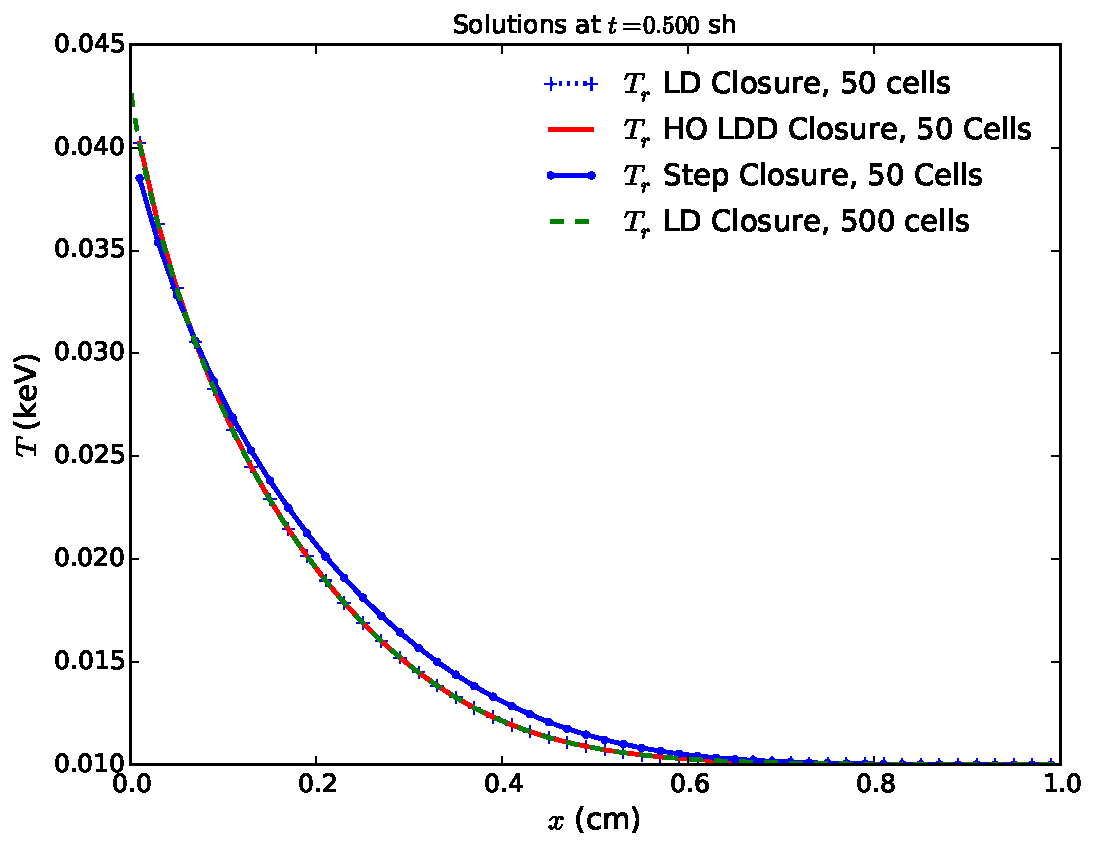
\includegraphics[width=0.99\linewidth]{smooth_compare.pdf}
    \caption{\label{fig:smooth_compare} Comparison of solutions for different spatial closures.}
\end{figure}

\begin{table}[H]

\end{table}

As the number of histories are increased, it is expected that the HO spatial closure will
be more accurate. In higher mesh counts and solutions this will be accurate, but a finer
mesh is needed to resolve the solution anyways, so there is not much hope of untieing the
solution.  No fixup is needed for the HO solution.




